iOSでは様々なフォントや色,行揃えを使用できる.読みやすさ,明快さ,一貫性が重要である\cite{developer.apple.com:design/human-interface-guidelines/ios/visual-design/typography/}.Dynamic Typeに対応すればユーザが文字サイズを変更した時も綺麗に見せることができる.また,ユーザが太字表示に切り替えた時の表示を確認するべきである\cite{developer.apple.com:design/human-interface-guidelines/ios/views/text-views/}\cite{developer.apple.com:design/design/human-interface-guidelines/ios/controls/labels/}.

特に重要なところはfont weight,size,colorを変更して強調する.可能ならば1つの書体とサイズを用いる\cite{developer.apple.com:design/human-interface-guidelines/ios/visual-design/typography/}.特別にカスタムフォントが必要な場合(ブランド戦略上やゲーム体験など)を除き,システムフォントを使い続けることが重要である.もしカスタムフォントを使う場合は小さい文字でも読みやすいものにする.

\begin{figure}[htbp]
    \begin{center}
        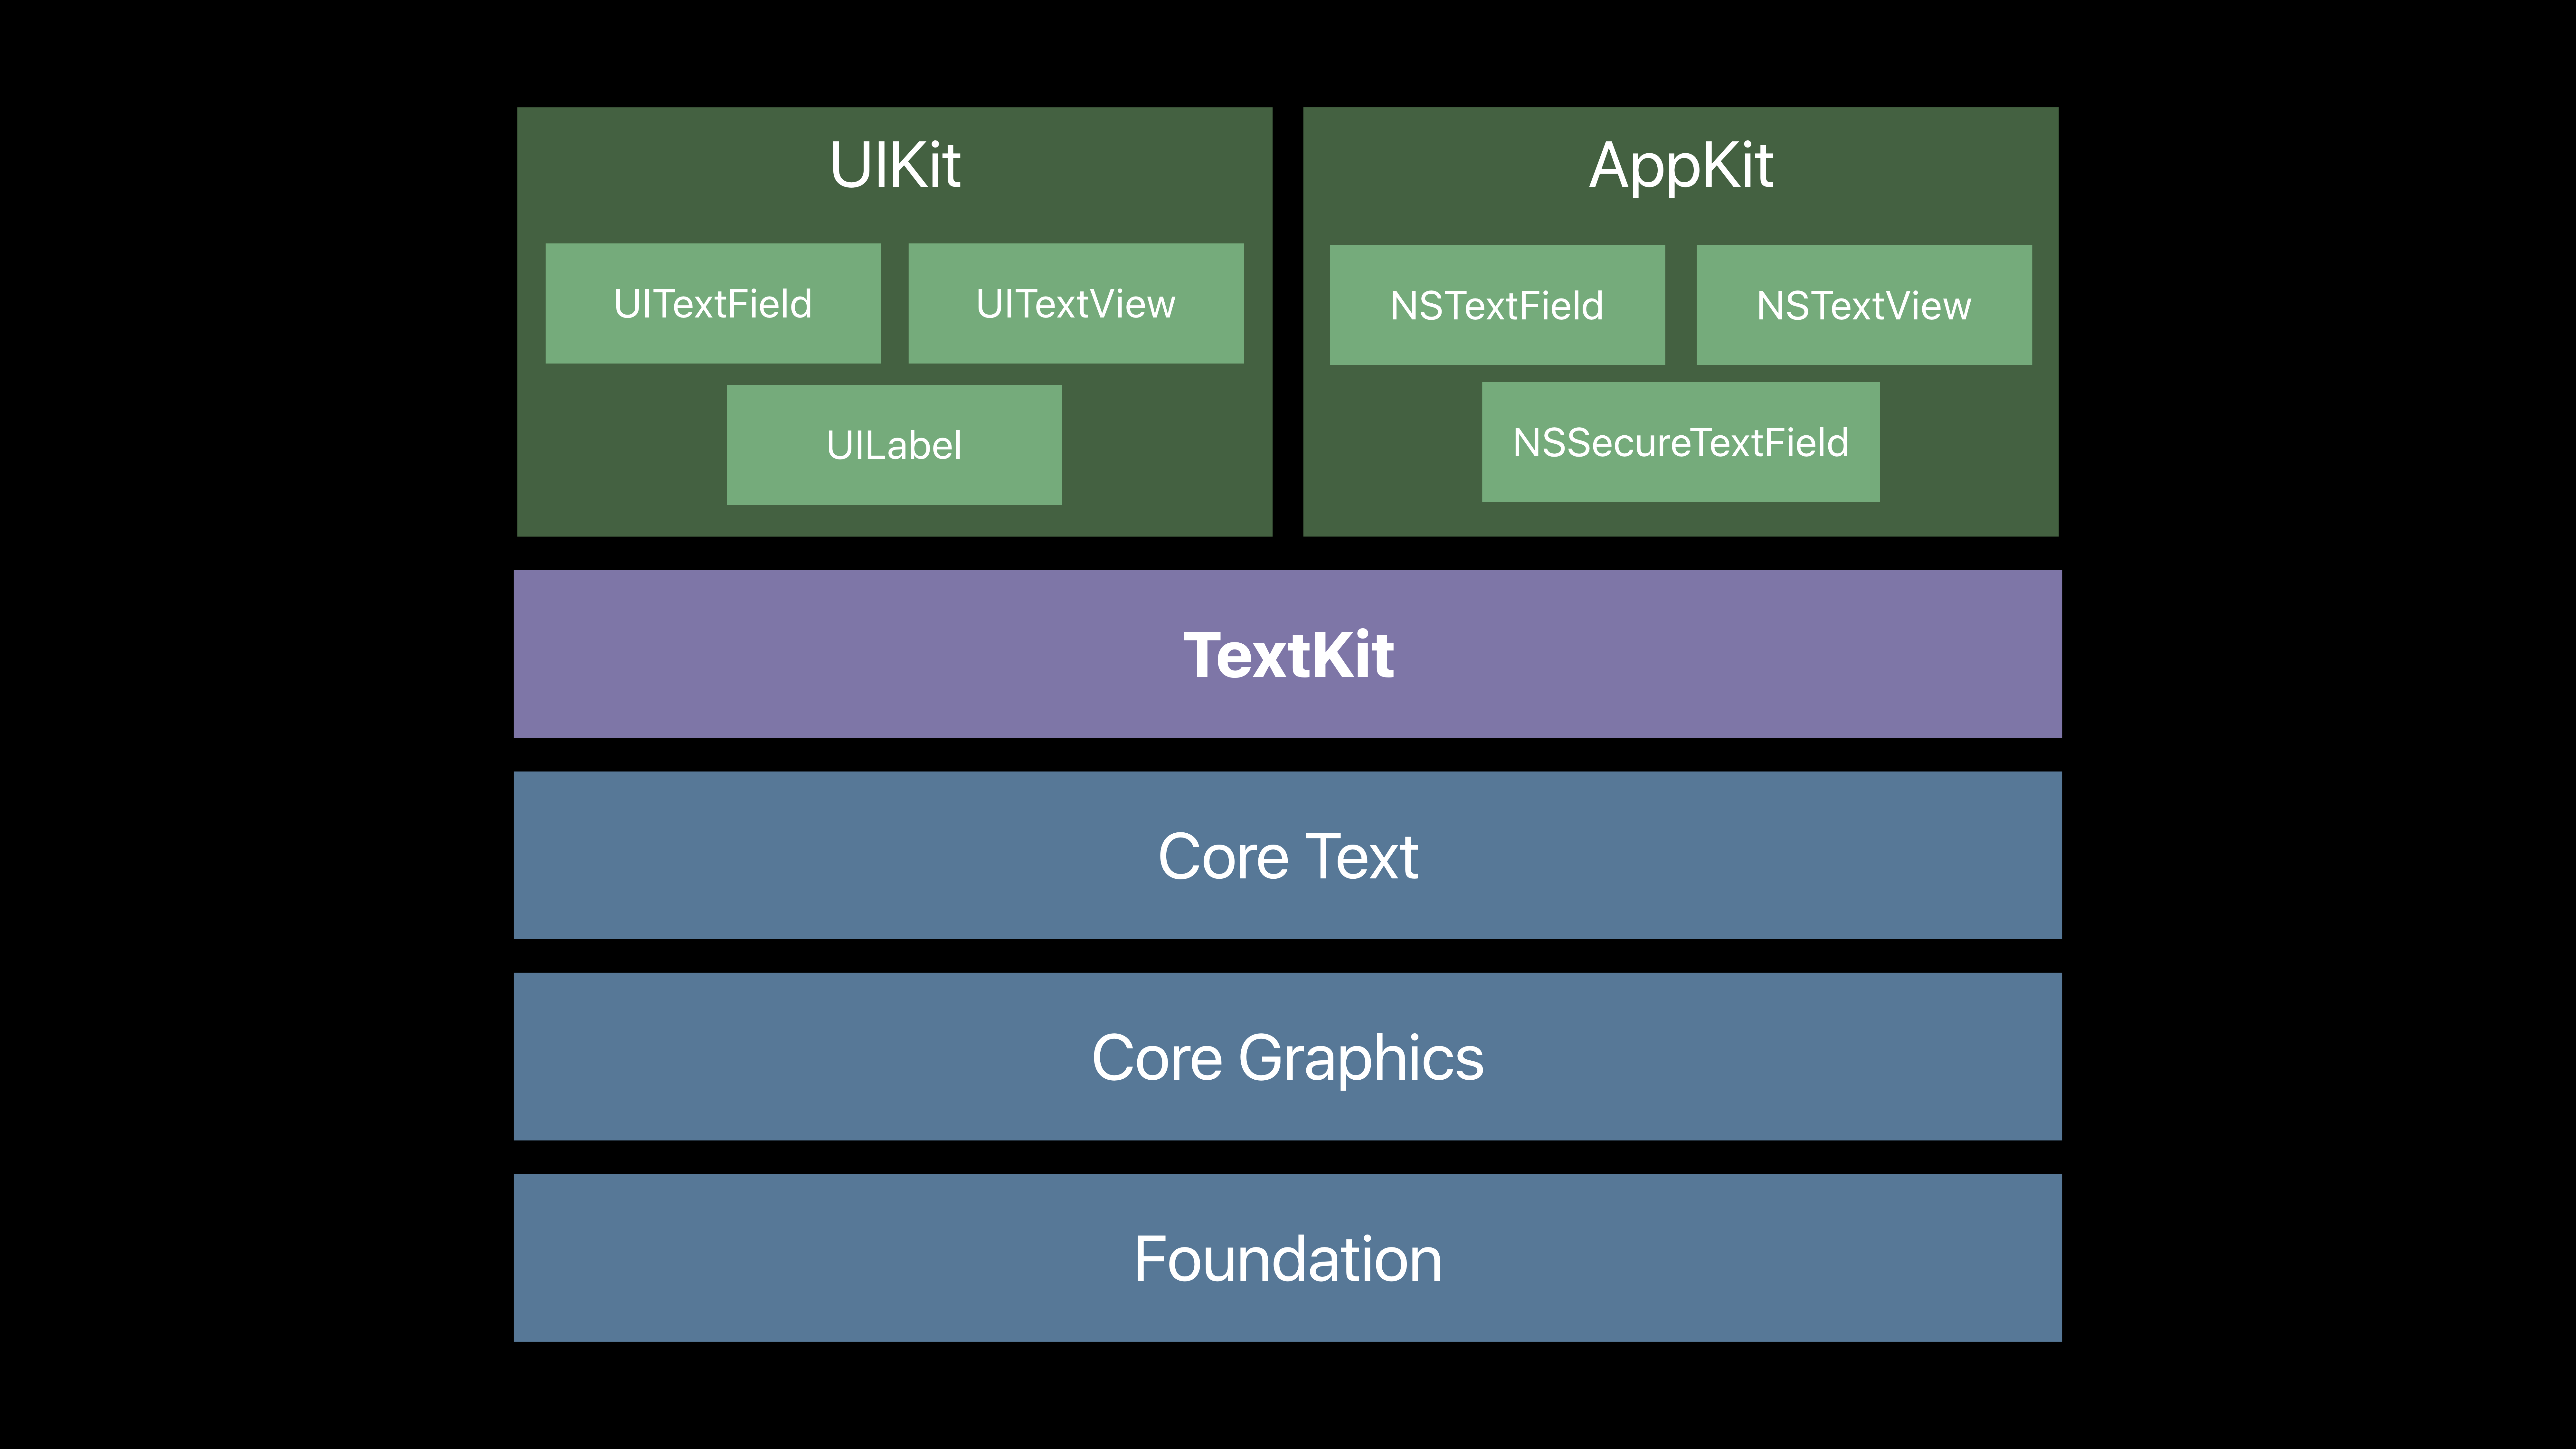
\includegraphics[width=0.8\linewidth]{images/textKit_hierarchie.png}
    \end{center}
    \caption{あとで消す}
\end{figure}

\begin{enumerate}
    \item TextKitとは
    \item Core Textとは
    \item Core Graphicsとは
\end{enumerate}

